\documentclass[]{article}
\usepackage{lmodern}
\usepackage{amssymb,amsmath}
\usepackage{ifxetex,ifluatex}
\ifnum 0\ifxetex 1\fi\ifluatex 1\fi=0 % if pdftex
\usepackage[T1]{fontenc}
\usepackage[utf8]{inputenc}
\setcounter{secnumdepth}{0}
\usepackage[table,xcdraw]{xcolor}
\usepackage[margin=1.5in]{geometry}
\usepackage[tableposition=top]{caption}
\usepackage{tabularx}
\usepackage{xcolor}
\usepackage{hyperref}
\usepackage{graphicx}
\hypersetup{
colorlinks=true,
linkcolor=blue,
filecolor=magenta,
urlcolor=cyan,
}



\title{Specyfikacja implementacyjna projektu indywidualnego \textbf{AiSD GR1}}
\author{Hubert Nakielski}
\date{Listopad 2020}

\begin{document}
    \maketitle


    \section{Informacje ogólne}
    Program napisany będzie w języku Java 14.0.1 i udostępniony jako plik o nazwie VaccineOptimizer w formacie .jar.\\
    Należy go uruchomić przez komendę: \textit{java -jar VaccineOptimizer.jar}.
    Program następnie poprosi o podanie ścieżki pliku wejściowego. Plik wyjściowy zostanie utworzony w folderze result.


    \section{Opis modułów}

    \subsection{Pakiet \textit{vaccine}}
    Pakiet zawierający wszystkie pakiety z kodem źródłowym.

    \subsection{Pakiet \textit{vaccine.file}}
    Odpowiedzialny za wszystkie czynności związane z plikami wejściowymi i wyjściowymi.

    \subsection{Pakiet \textit{vaccine.calculations}}
    Odpowiada za liczenie najtańszej konfiguracji zakupionych szczepionek.

    \subsection{Pakiet \textit{vaccine.objects}}
    Zawiera klasy odpowiedzialne za tworzenie obiektów takich jak: Producent, Apteka, Połączenie (między apteką, a producentem)

    \subsection{Folder \textit{vaccine.result}}
    W tym miejscu będzie zapisywany plik wyjściowy


    \section{Opis klas }

    \subsection{Klasa \textit{ConfigurationIO}}
    Zawiera się w module \textit{file}, czyta plik wejściowy, tworzy listy aptek, producentów i połączeń. Tworzy plik wyjściowy z konkretną konfiguracją. Zawiera 3 zmienne, 2 metody dostępowe i jedną metodę modyfikującą:\\

    $\bullet$ \verb|path|: String

    $\bullet$ \verb|manufacturerList|: List<Manufacturer>

    $\bullet$ \verb|pharmacyList|: List<Pharmacy>\\

    $ \blacktriangleright $ \verb|getManufacturerList()|: List<Manufacturer>

    $ \blacktriangleright $ \verb|getPharmacyList()|: List<Pharmacy>

    $ \blacktriangleright $ \verb|setPath()|: void

    Metody w klasie:

    \subsubsection{loadFromFile(String filePath)}
    Metoda odpowiedzialna za czytanie pliku wejściowego.\\
    Wartość zwracana: \verb|void|

    \subsubsection{isPharmaciesInfo(String line)}
    Sprawdza czy pod sprawdzaną linijką znajdują się informacje o aptekach.\\
    Wartość zwracana: \verb|boolean|

    \subsubsection{isManufacturersInfo(String line)}
    Sprawdza czy pod sprawdzaną linijką znajdują się informacje o producentach.\\
    Wartość zwracana: \verb|boolean|

    \subsubsection{isConnectionsInfo(String line)}
    Sprawdza czy pod sprawdzaną linijką znajdują się informacje o połączeniach.\\
    Wartość zwracana: \verb|boolean|

    \subsubsection{parseManufacturersLine(String line)}
    Dodaje producentów i ich dane do listy zgodnie z plikiem wejściowym.\\
    Wartość zwracana: \verb|void|

    \subsubsection{parsePharmaciesLine(String line)}
    Dodaje apteki i ich dane do listy zgodnie z plikiem wejściowym.\\
    Wartość zwracana: \verb|void|

    \subsubsection{parseConnectionsLine(String line)}
    Dodaje połączenia do listy zgodnie z plikiem wejściowym.\\
    Wartość zwracana: \verb|void|

    \subsubsection{saveToFile(List<Pharmacy> pharmacyList)}
    Metoda odpowiedzialna za wpisywanie gotowej konfiguracji do pliku wyjściowego.\\
    Wartość zwracana: \verb|void|

    \subsection{Klasa \textit{Manufacturer}}
    Występuje w module \textit{object}.
    Zawiera 5 zmiennych, ich metody dostępowe oraz jedną metodę modyfikującą:

    $\bullet$ \verb|id|: int

    $\bullet$\verb| name|: String

    $\bullet$ \verb|daily_production|: int

    $\bullet$ \verb|connectionList|: List<Connection>

    $\bullet$ \verb|vamFactor|: int\\

    $ \blacktriangleright $ \verb|getId()|: int

    $ \blacktriangleright $ \verb|getName()|: String

    $ \blacktriangleright $ \verb|getDailyProduction()|: int

    $ \blacktriangleright $ \verb|getConnectionList()|: List<Connection>

    $ \blacktriangleright $\verb|getVamFactor()|: int\\

    $ \blacktriangleright $\verb|setVamFactor(int vamFactor)|: void

    \subsection{Klasa \textit{Pharmacy}}
    Występuje w module \textit{object}.
    Zawiera 5 zmiennych, ich metody dostępowe oraz jedną metodę modyfikującą:

    $\bullet$ \verb|id|: int

    $\bullet$ \verb|name|: String

    $\bullet$ \verb|need|: int

    $\bullet$ \verb|connectionList|: List<Connection>

    $\bullet$ \verb|vamFactor|: int\\

    $ \blacktriangleright $ \verb|getId()|: int

    $ \blacktriangleright $ \verb|getName()|: String

    $ \blacktriangleright $ \verb|getNeed()|: int

    $ \blacktriangleright $ \verb|getConnectionList()|: List<Connection>

    $ \blacktriangleright $\verb|getVamFactor()|: int\\

    $ \blacktriangleright $\verb|setVamFactor(int vamFactor)|: void\\

    Dodatkowo klasa ta zawiera metodę:

    \subsubsection{addConnection(Manufacturer manufacturer,Pharmacy pharmacy, int quantity, double price)}
    Dodaje połączenie do listy połączeń (używana jest podczas czytania pliku)\\
    Wartość zwracana: \verb|void|

    \subsection{Klasa \textit{Connection}}
    Występuje w module \textit{object}.
    Zawiera 4 zmienne, ich metody dostępowe oraz jedną metodę modyfikującą:

    $\bullet$ \verb|manufacturer|: Manufacturer

    $\bullet$ \verb|pharmacy|: Pharmacy

    $\bullet$ \verb|quantity|: int

    $\bullet$ \verb|price|: double\\

    $ \blacktriangleright $ \verb|getManufacturer|: Manufacturer

    $ \blacktriangleright $ \verb|getPharmacy()|: Pharmacy

    $ \blacktriangleright $\verb|getQuantity()|: int

    $ \blacktriangleright $\verb|getPrice()|: double\\

    $ \blacktriangleright $\verb|setQuantity(int quantity)|: void\\

    \subsection{Klasa \textit{VAM}}
    Zawiera się w module \textit{calculations}, liczy konfigurację o najmniejszym koszcie używając metody VAM (Vogel's approximation method).
    Zawiera 4 zmienne oraz konstruktor:\\

    $\bullet$ \verb|configurationIO|: ConfigurationIO

    $\bullet$ \verb|manufacturerList|: List<Manufacturer>

    $\bullet$ \verb|pharmacyList|: List<Pharmacy>

    $\bullet$ \verb|connectionList|: List<Connection>\\

    $ \blacktriangleright $\verb|Pharmacy(int id, String name, int need)|\\


    Metody w klasie:

    \subsubsection{minimizeCost(List<Pharmacy> pharmacyList, List<Manufacturer> manufacturerList)}
    Metoda odpowiedzialna za liczenie minimalnego kosztu.\\
    Wartość zwracana: \verb|List<Connection>|

    \subsubsection{calculateVAMFactor()}
    Metoda odpowiedzialna za obliczenie współczynnika VAM dla każdej apteki i dla każdego producenta. \\
    Wartość zwracana: \verb|void|

    \subsubsection{findGreatestVAMFactor()}
    Znajduje najwyższy współczynnik VAM i zwraca daną aptekę lub producenta, w której on występuje.\\
    Wartość zwracana: \verb|Object|

    \subsubsection{adjustPossibleQuantity(Pharmacy pharmacy, Manufacturer manufacturer)}
    Ustala najwyższą możliwą ilość szczepionek dostarczanej z danego producenta do danej apteki, uwzględniając:

    - zapotrzebowanie apteki,

    - dzienną produkcję producenta,

    - dzienną maksymalną liczbę dostarczanych szczepionek od danego producenta do danej apteki ( wynikające z umowy )\\
    Wartość zwracana: \verb|int|

    \subsubsection{generateConfigurationToFile()}
    Wywołuje metodę \textit{saveToFile(List<Pharmacy>)} z klasy ConfigurationIO podając przy tym gotową listę aptek \verb|connectionList| ( zawierającą listę połączeń w odpowiedniej już konfiguracji)\\
    Wartość zwracana: \verb|void|


    \section{Logika liczenia najtańszej konfiguracji}
    \newcommand\tab[1][1cm]{\hspace*{#1}}
    Liczenie odbywać się będzie używając metody VAM. Dla tej metody utworzymy dodatkowe zmienne (współczynnik VAM) dla każdego obiektu ( apteka / producent ).\\\\
    \textbf{1. Liczę wspólczynnik VAM}
    
    1.1 dla każdego obiektu sprawdzam cenę poszczególnego połączenia, które jest związane z danym obiektem)
    
    1.2 wybieram minimum z tych cen;
    
    1.3 wybieram drugie minimum z tych cen;
    
    1.4 obliczam różnicę z tych dwóch minimów.\\\\ 
    \textbf{2. Znajduję największy współczynnik}
    
    2.1 wybieram maximum ze współczynników wszystkich obiektów;
    
    2.2 zapamiętuję aptekę, dla której ten współczynnik wystąpił.\\\\
    \textbf{3. Ustalam najtańszą konfigurację dla podanej apteki}
    
    3.1 dla zapamiętanej apteki znajduję połączenie, dla którego cena szczepionki będzie najniższa i zapamiętuję je;
    
    3.2 ustalam najwyższą ilość szczepionek dla zapamiętanego połączenia, spełniającą warunki:\\
    \tab •suma kupionych przez aptekę szczepionek nie przekracza dziennego \\\tab zapotrzebowania\\
    \tab •suma sprzedanych przez producenta szczepionek nie przekracza dziennej produkcji\\
     \tab •ilość kupionych/sprzedanych szczepionek w danym połączeniu nie przekracza\\\tab  dziennej maksymalnej liczby dostarczanych szczepionek przez producenta do apteki
     
     3.3 dla tej samej apteki znajduję drugie najtańsze połączenie, dla którego cena szczepionki będzie najniższa i zapamiętuję je;
     
     3.4 ponownie wykonuję punkt 3.2;
     
     3.5 kończę ustalanie najtańszej konfiguracji dla tej apteki, gdy suma kupionych przez aptekę szczepionek będzie równa dziennemu zapotrzebowaniu.\\
     \textbf{4. Wracam do punktu 1.  bez uwzględniania już zapełnionych aptek}
     
     4.1 kończę, gdy każda apteka ma już ustaloną konfigurację
     
     
    \section{Testowanie}
 
    \subsection{Użyte narzędzia}
    Do testowania użyję narzędzia JUnit. W testach sprawdzę poprawne działanie poszczególnych metod. Wyszukiwanie optymalnego rozwiązania w programie przetestuję manualnie dla różnych zestawów danych - w programie Microsoft Excel przygotowałem gotowy arkusz optymalizujący dane wejściowe inną metodą. Planuję porównać ze sobą oba wyniki. Przetestuję też wyrzucanie odpowiednich błędów dla niepoprawnego pliku wejściowego.

    \subsection{Konwencja}
    Nazewnictwo metod testujących powinno być zgodne z testowaną funkcjonalnością. Czyli nazwa metody powinna jasno sygnalizować co program powinien zwracać i dla jakiego scenariusza. Dla przykładu:
    
    źle $ \Rightarrow $ \verb|testLoadFromFile()|
    
    dobrze $ \Rightarrow $ \verb|should_GenerateListOfPharmacies_when_InputFileIsCorrect()|\\\\
    Każdy test powinien być napisany zgodnie z konwencją:
    
   \verb| \\given|
    
    \verb| \\when|
    
    \verb| \\then|

    \subsection{Warunki brzegowe}
    DODAJ


    \section{Diagram klas}

    \noindent
    \makebox[\textwidth]{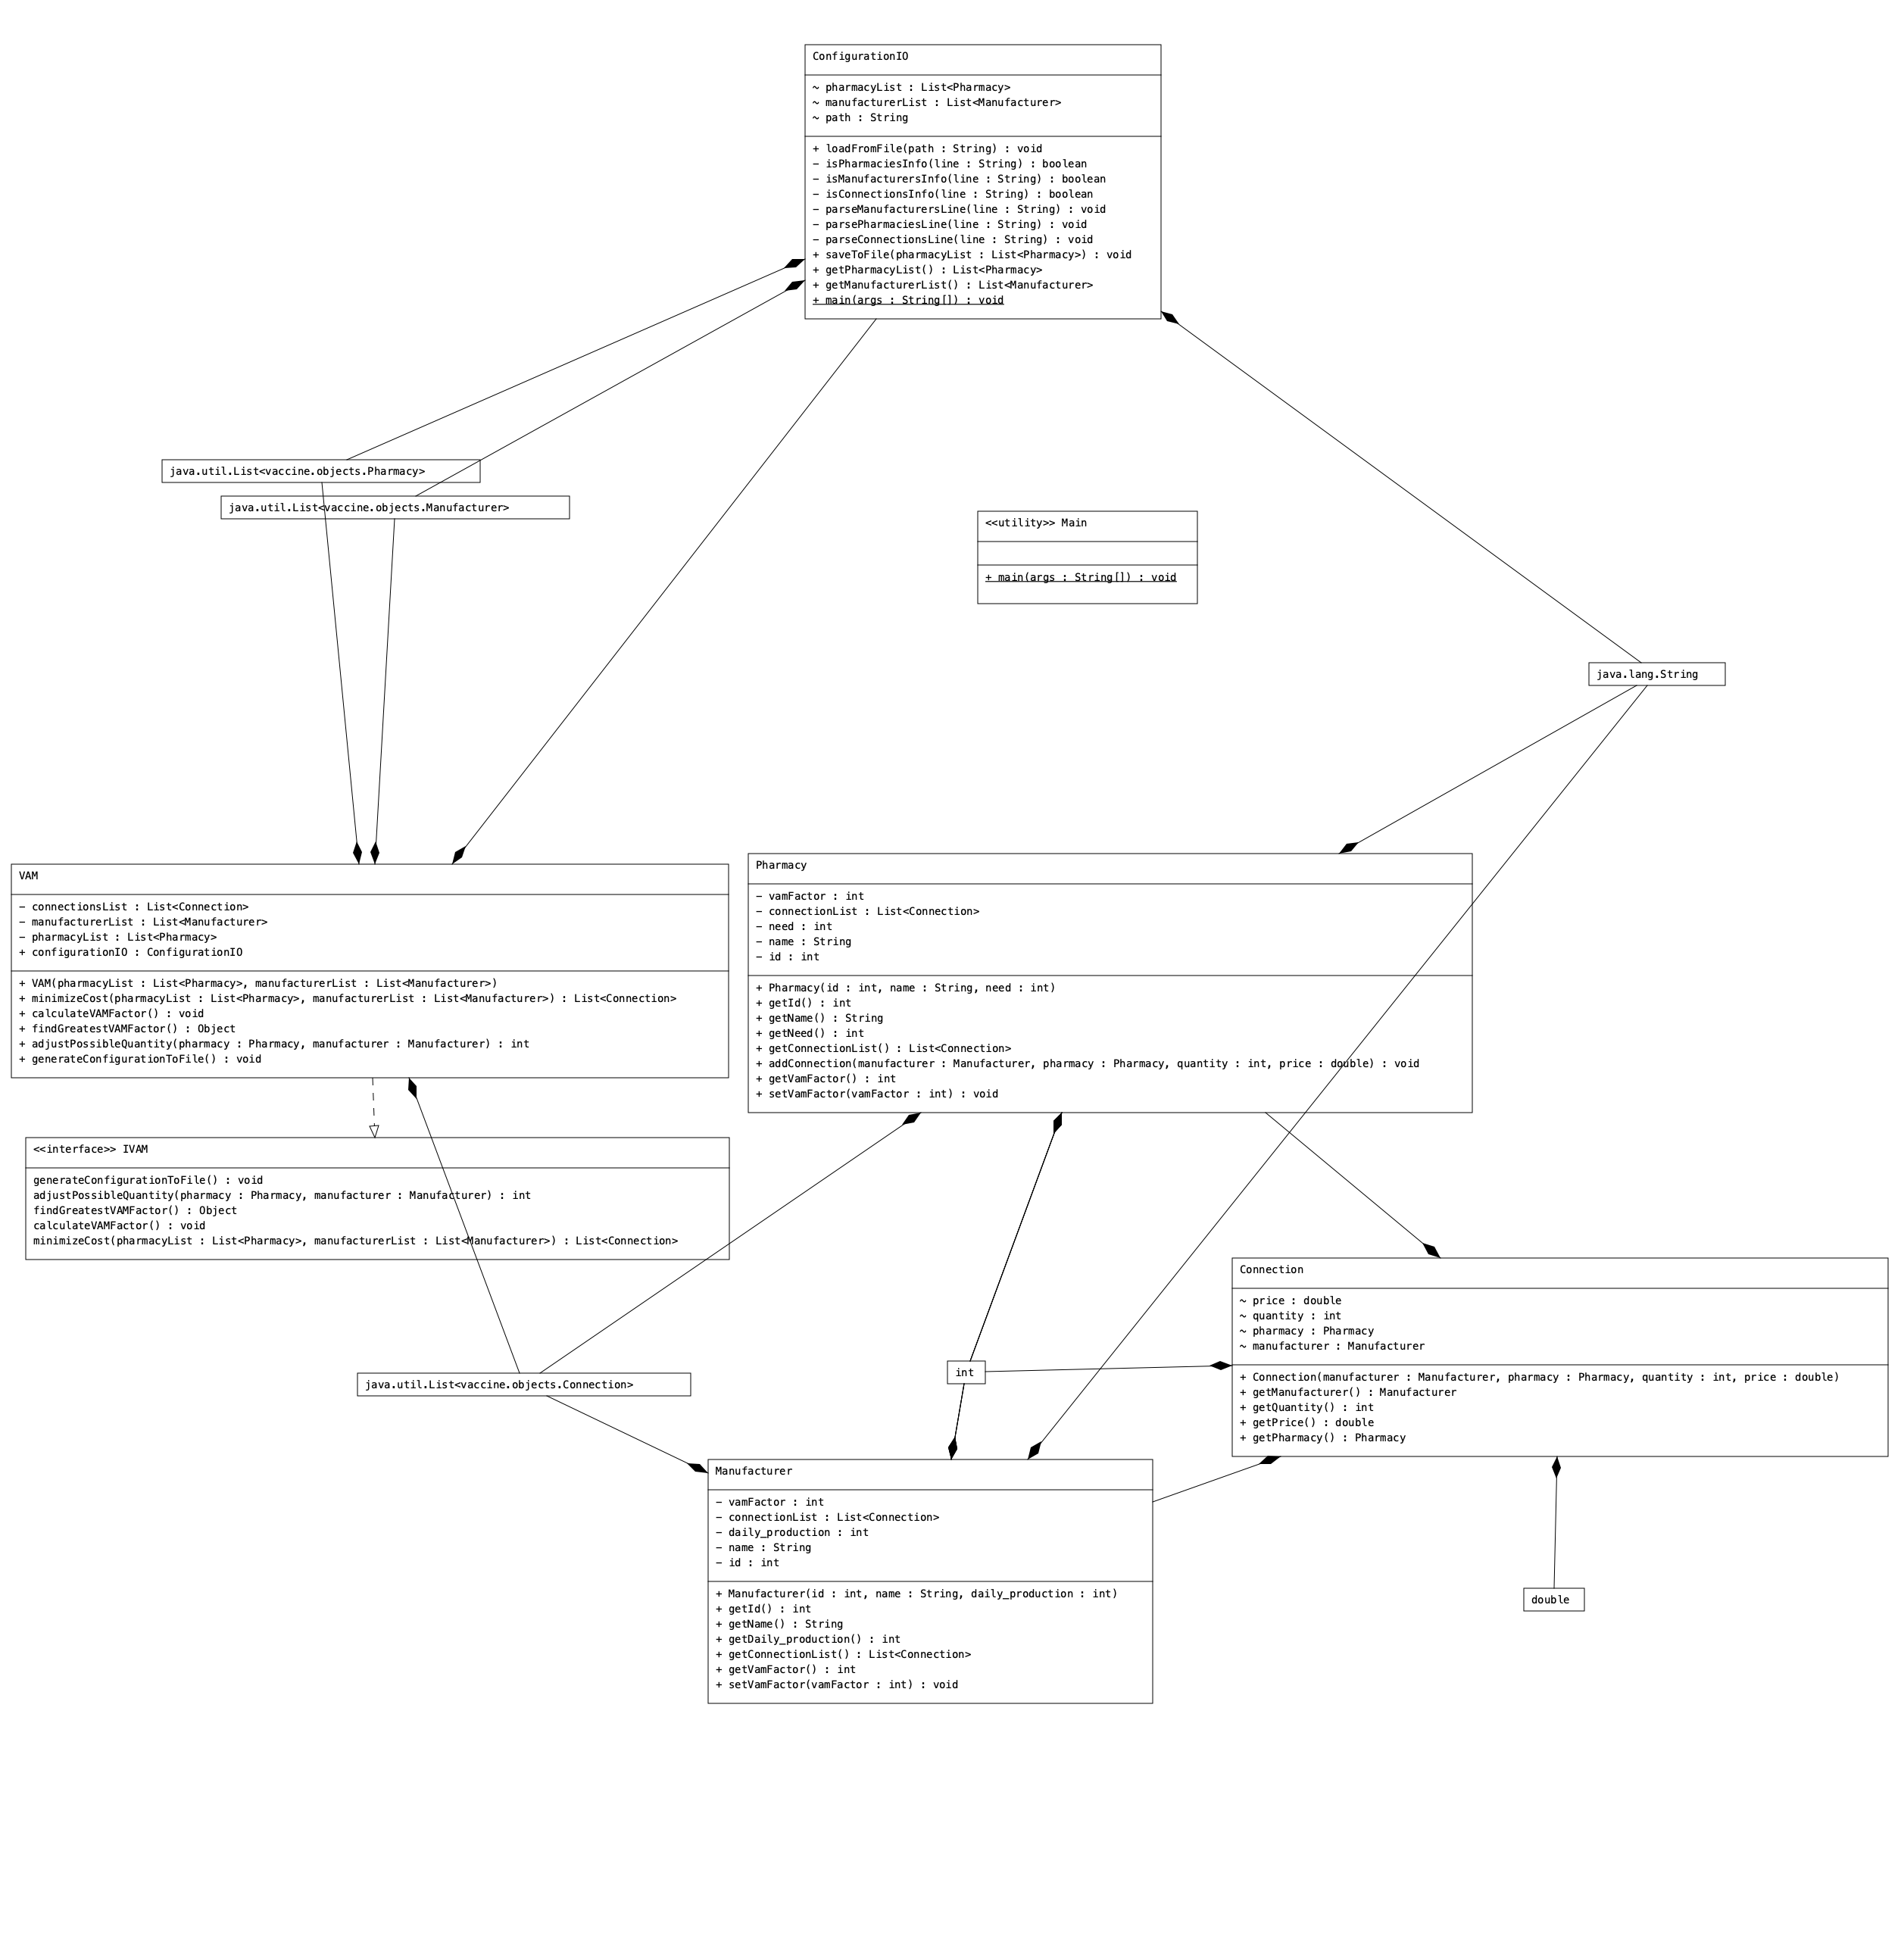
\includegraphics[width = 1.5\linewidth]{Class diagram.png}}

\end{document}